\chapter{行列式}

\section{Overview}
\begin{figure}[h]
	\centering
	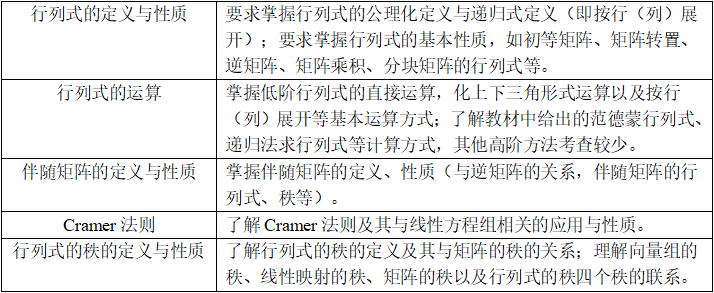
\includegraphics[scale=0.58]{7.png}
\end{figure}

\section{行列式的定义与性质}
很多教材采用“逆序数”定义行列式(感兴趣的同学可以参考丘维声《高等代数》等教材),但是本教材未提及,因此
我们作为复习课也不展开描述。本教材使用公理化定义(使用一些规则描述)并讲解了
递归式定义(按行(列)展开)。

\subsection{公理化定义}
\begin{definition}
	数域$\mathbf{F}$上的一个$n$阶行列式是取值于$\mathbf{F}$的$n$个$n$维向量
	$\alpha_1,\alpha_2,\dots,\alpha_n \in \mathbf{F}^n$的一个函数,且$\forall \alpha_i,\beta_i \in \mathbf{F}^n$
	和$\forall \lambda \in \mathbf{F}$,满足下列规则:
	
	\textup{1}.(齐性)$D(\alpha_1,\dots,\lambda\alpha_i,\dots,\alpha_n)=\lambda D(\alpha_1,\dots,\alpha_i,\dots,\alpha_n)$\textup{;}

	\textup{2}.(加性,与\textup{1}合称线性性)
	
	$D(\alpha_1,\dots,\alpha_i+\beta_i,\dots,\alpha_n)=D(\alpha_1,\dots,\alpha_i,\dots,\alpha_n)+D(\alpha_1,\dots,\beta_i,\dots,\alpha_n)$\textup{;}

	\textup{3}.(反对称性)$D(\alpha_1,\dots,\alpha_i,\dots,\alpha_j,\dots,\alpha_n)=-D(\alpha_1,\dots,\alpha_j,\dots,\alpha_i,\dots,\alpha_n)$\textup{;}

	\textup{4}.(规范性)$D(e_1,e_2,\dots,e_n)=1$.
\end{definition}
在公理化定义中,我们将行列式定义为一个满足特定的运算性质的从列向量组合到数的函数。
事实上,公理化定义从是逆序数定义可以推导出的行列式的运算性质,教材采用这种定义避开了繁琐的说明。
除此之外,我们不难看出公理化定义可以形象地理解为对$n$维空间中体积的定义,
对几何意义感兴趣的同学可以参考3b1b《线性代数的本质》系列视频相关内容。
\begin{example}
	使用定义$1$验证下述命题的正确性:

	\textup{1}. 若行列式有一列为零向量,则行列式的值等于$0$.

	\textup{2}. 若行列式有两列元素相同,则行列式的值等于$0$.

	\textup{3}. 若行列式有两列元素成比例,则行列式的值等于$0$.

	\textup{4}. 对行列式做倍加列变换,行列式的值不变.

	\textup{5}. 若$\alpha_1,\alpha_2,\dots,\alpha_n$线性相关,则$D(\alpha_1,\alpha_2,\dots,\alpha_n)=0$.
\end{example}

\begin{example}
	设向量$\alpha_1$,$\alpha_2$,$\beta_1$,$\beta_2$为三维列向量,又$A=(\alpha_1,\alpha_2,\beta_1)$,$B=(\alpha_1,\alpha_2,\beta_2)$,
	且$|A|=3$,$|B|=2$,求$|2A+3B|$.
\end{example}

\subsection{递归式定义}
首先需要回顾余子式和代数余子式的概念:
\begin{definition}
	在$n$阶行列式$D=|a_{ij}|_{n \times n}$中,去掉元素$a_{ij}$所在的第$i$行和第$j$列的所有元素
	而得到的$n-1$阶行列式称为元素$a_{ij}$的余子式,记作$M_{ij}$,并把数$A_{ij}=(-1)^{i+j}M_{ij}$
	称为元素$a_{ij}$的代数余子式.
\end{definition}
注意,虽然余子式和代数余子式在名称中含有式,但实际上他们是一个值。实际上行列式也称为“式”,但这些“式”
只是形状上有个形式,实际上只是一个值。
\begin{example}
	根据定义$2$计算行列式$\begin{vmatrix}
		2 & 1 & 3 \\
		-1 & 0 & 2 \\
		1 & 5 & -2
	\end{vmatrix}$每个元素的余子式和代数余子式.
\end{example}

接下来我们便可以给出递归式定义:
\begin{definition}
	设$D=|a_{ij}|_{n \times n}$,则
	\begin{equation}
		D=\sum_{k=1}^{n}a_{kj}A_{kj}=a_{1j}A_{1j}+a_{2j}A_{2j}+\dots+a_{nj}A_{nj},\ j=1,2,\dots,n
	\end{equation}
	\begin{equation}
		D=\sum_{k=1}^{n}a_{ik}A_{ik}=a_{i1}A_{i1}+a_{i2}A_{i2}+\dots+a_{in}A_{in},\ i=1,2,\dots,n
	\end{equation}
\end{definition}
其中$A_{ij}$即为定义2给出的代数余子式,(1)式称为$D$对第$j$列的展开式,(2)式称为$D$对第$i$行的展开式。这一定义与公理化定义的
等价性不难证明。事实上,这一定义被称为递归式定义的原因是显然的(如果在程序设计课程中已经学习过递归的概念),它使用$n-1$阶行列式定义$n$阶行列式,我们对任意$n$阶行列式
都可以递归展开到1阶,从而得到最终行列式计算结果。
\begin{example}
	利用定义$3$计算例$3$中的行列式,可以行列展开均使用并在上述公式中选取不同$i$和$j$以熟悉定义$3$,并注意体会递归式定义的含义.
\end{example}

递归式定义有一个相关的结论如下:
\begin{theorem}
	$n$阶行列式$D=|a_{ij}|_{n \times n}$的某一行(列)元素与另一行(列)相应元素的代数余子式
	的乘积之和等于$0$,即
	\begin{equation}
		\sum_{k=1}^{n}a_{kj}A_{ki}=a_{1j}A_{1i}+a_{2j}A_{2i}+\dots+a_{nj}A_{ni}=0,\ j \neq i
	\end{equation}
	\begin{equation}
		\sum_{k=1}^{n}a_{jk}A_{ik}=a_{j1}A_{i1}+a_{j2}A_{i2}+\dots+a_{jn}A_{in}=0,\ j \neq i
	\end{equation}
\end{theorem}
我们若将行列式第$j$列元素替换为第$i$列元素,那么上述(3)式根据定义3就是在求替换后的行列式,
并且有两列元素相同的行列式为0,我们便可以轻松地证明(3),实际上(4)同理也可证明。同学们可能
对(1)-(4)式繁杂的下标感到陌生,因此安排了例2-4希望大家熟悉这些公式.
\begin{example}
	对例$3$中的矩阵验证定理$1$的正确性.
\end{example}
这一节中行列式是按照一行(列)展开的,若按多行(列)展开则需要相应的拉普拉斯定理,感兴趣的同学可以了解。
\subsection{行列式的常用性质}
设$A,B \in \mathbf{F}^{n \times n}$,$k \in \mathbf{F}$,则

1. 一般情况下,$|A \pm B| \neq |A|\pm|B|$;

2. $|kA|=k^n|A|$;

3. $A$可逆$\iff |A| \neq 0$;

4. 初等矩阵行列式(注意初等矩阵不分行列,左乘右乘区分初等行列变换):$|E_{ij}|=-1$,$|E_i(c)|=c$,$|E_{ij}(k)|=1$;

5. 利用4中的结论可以得到$|A^\mathrm{T}|=|A|$:

6. 利用4中的结论可以得到$|AB|=|A||B|$,$|A^k|=|A|^k$;

7. 利用4中的结论(求出初等矩阵逆矩阵行列式)可以得到若$A$可逆,则$|A^{-1}|=|A|^{-1}$.

以上性质都可以基于定义或上述其他性质得到,下面介绍的性质需要用到“打洞法”(分块矩阵初等变换)
来证明:

1. $\begin{vmatrix}
	A & O \\ O & B
\end{vmatrix} = \begin{vmatrix}
	A & O \\ C & B
\end{vmatrix} = \begin{vmatrix}
	A & D \\ O & B
\end{vmatrix} = |A||B|,\ \begin{vmatrix}
	O & A \\ B & C
\end{vmatrix} = (-1)^{kr}|A||B|$;

2. 当$A$可逆时,有$\begin{vmatrix}
	A & B \\ C & D
\end{vmatrix} = |A||D-CA^{-1}B|$,当$D$可逆时,有
$\begin{vmatrix}
	A & B \\ C & D
\end{vmatrix} = |D||A-BD^{-1}C|$,当$B$可逆时,有
$\begin{vmatrix}
	A & B \\ C & D
\end{vmatrix} = (-1)^{mn}|B||C-DB^{-1}A|$,当$C$可逆时,有
$\begin{vmatrix}
	A & B \\ C & D
\end{vmatrix} = (-1)^{mn}|C||B-AC^{-1}D|$;

3. 设$A$和$B$分别是$n \times m$和$m \times n$矩阵,则$|E_n \pm AB|=|E_m \pm BA|$,且
$|\lambda E_n \pm AB|=\lambda^{n-m}|\lambda E_m \pm BA|(n \ge m)$.

还有一部分由这些性质可以推导的其他性质将出现在C组习题中供参考。这部分主要是技巧性内容,可以选择性完成。
\subsection{习题}
\centerline{\heiti A组}
\begin{enumerate}
	\item 设$\alpha_1,\alpha_2,\alpha_3$为三维列向量,令$A=(\alpha_1,\alpha_2,\alpha_3)$,
	且$|A|=2$,求$|\alpha_1+\alpha_2+\alpha_3,\alpha_1+3\alpha_2+9\alpha_3,\alpha_1+4\alpha_2+16\alpha_3|$.
	\item 求证以下命题:
	
	(1)奇数阶反对称矩阵不可逆;
	
	(2)若$A$是$n$阶可逆对称矩阵,$B$是$n$阶反对称矩阵,则当$n$为奇数时,齐次线性方程组$(AB)X=O$有非零解.
\end{enumerate}

\centerline{\heiti B组}
\begin{enumerate}
	\item 设$D=\begin{vmatrix}
		3 & 0 & 4 & 1 \\ 2 & 3 & 1 & 4 \\ 0 & -7 & 8 & 3 \\ 5 & 3 & -2 & 2
	\end{vmatrix}$,求

	(1)$A_{21}+A_{22}+A_{23}+A_{24}$;

	(2)$A_{31}+A_{33}$;

	(3)$M_{41}+M_{42}+M_{43}+M_{44}$;
	\item 求参数 $a,\ b$  的值,使得 $\begin{vmatrix}1 & 1 & 1 \\ x & y & z \\u & v & w\end{vmatrix}=1,\ \begin{vmatrix}1 & 2 & -5 \\ x & y & z \\u & v & w\end{vmatrix}=2,\ \begin{vmatrix}2 & 3 & b \\ x & y & z \\u & v & w\end{vmatrix}=a$ 都成立,并求$\begin{vmatrix}x & y & z \\ 1 & -1 & 5 \\u & v & w\end{vmatrix}$.
	\item 设$A$,$B$为三阶矩阵,且$|A|=3$,$|B|=2$,且$|A^{-1}+B|=2$,求$|A+B^{-1}|$.
	\item 设$A$为$n$阶正交矩阵,即$AA^\mathrm{T}=A^\mathrm{T}A=E$,且$|A|<0$,证明:$|E+A|=0$.
	\item 已知齐次线性方程组$$\begin{cases}
		a_{11}x_1+a_{12}x_2+\cdots+a_{1n}x_n=0 \\
		a_{21}x_1+a_{22}x_2+\cdots+a_{2n}x_n=0 \\
		\cdots \\
		a_{n-1,1}x_1+a_{n-1,2}x_2+\cdots+a_{n-1,n}x_n=0
	\end{cases},$$设$M_j(j=1,2,\cdots,n)$表示$A$划掉第$j$列所得的$n-1$阶子式,证明:

	(1)$(M_1,-M_2,\cdots,(-1)^{n-1}M_n)$是方程组的一个解;

	(2)若$r(A)=n-1$,则方程组的解全是$(M_1,-M_2,\cdots,(-1)^{n-1}M_n)$的倍数.
\end{enumerate}

\centerline{\heiti C组}
\begin{enumerate}
	\item 设$A$,$B$,$C$,$D$均为$n$阶方阵,且$AC=CA$,证明:
	$$\begin{vmatrix}
		A & B \\ C & D
	\end{vmatrix} = |AD-CB|.$$

	\item 设$A$为$n$阶可逆矩阵,$\alpha$,$\beta$为$n$维列向量,证明:
	$$|A+\alpha\beta^{\mathrm{T}}|=|A|(1+\beta^\mathrm{T}A^{-1}\alpha).$$
	\item 设$A$,$B$均为$n$阶方阵,证明:
	$$\begin{vmatrix}
		A & B \\ B & A
	\end{vmatrix} = |A+B||A-B|.$$
	\item 设$A$,$B$,$C$,$D$均为$n$阶方阵,且$r\begin{pmatrix}
		A & B \\ C & D
	\end{pmatrix}=n$,证明:
	$$\begin{vmatrix}
		|A| & |B| \\ |C| & |D|
	\end{vmatrix} = 0.$$
	\item $^*$(对角占优)设$A=(a_{ij})_{n \times n}$是一个$n$级矩阵,证明:
	
	(1)若$A$为复矩阵,且$|a_{ii}|>\sum_{j \neq i}|a_{ij}|$,那么$|A|\neq 0$;

	(2)若$A$为实矩阵,且$a_{ii}>\sum_{j \neq i}|a_{ij}|$,那么$|A|>0$;

	(3)(推论)存在充分大的实数$M$,使得$t>M$时,$tE+A$可逆.
\end{enumerate}

\section{行列式的运算}
\subsection{概述}
本节内容按照往年经验不是考试重点,实际上行列式这章在往年单独出现的
频率较低,一般都在求解特征值或者作为判断可逆等情况下作为结论使用,但是我们仍然需要掌握基本的行列式计算方法,
至少教材中给出的例题需要熟悉。

一般而言行列式的计算方法有根据定义求解(包括逆序数定义(包括低阶行列式直接计算公式)、公理化定义和递归式定义(或拉普拉斯定理))、
高斯消元法化为上三角矩阵求解、拆分法(大拆分法、小拆分法)求解、加边法(升阶法)求解、特殊行列式求解
(如“箭形”行列式,循环行列式,范德蒙行列式)、递推法求解、数学归纳法求解(这两种方法一般用于大对角形)、
打洞法求解以及利用特征值求解等,具体方法不在此展开,一般教辅书上都有详细介绍,因为这不是线性代数荣誉课
重点内容,因此我们不详细说明这些方法,只在下面的习题中给出几个例子。

\subsection{习题}
注:本节习题只给出少量练习回顾基本方法以及给出少量特殊的例子,如果需要系统性练习高阶方法的建议参考此前陈小川学长的行列式授课资料
或其他参考书等。

\centerline{\heiti A组}
\begin{enumerate}
	\item 推导二阶行列式与三阶行列式直接计算的一般公式.
	\item 利用行列式的定义计算对角矩阵,副对角矩阵(即只有副对角线元素非0)以及上(下)三角矩阵行列式.
	\item 利用初等变换化对角矩阵的方法求四阶行列式$\begin{vmatrix}
		1 & 2 & -2 & 3 \\ -1 & -2 & 4 & -2 \\ 0 & 1 & 2 & -1 \\ 2 & 3 & -3 & 10
	\end{vmatrix}$.
	\item 计算行列式$\begin{vmatrix}
		\alpha & \beta & \gamma \\
		\gamma & \alpha & \beta \\
		\beta & \gamma & \alpha
	\end{vmatrix}$,其中$\alpha$,$\beta$,$\gamma$是方程$x^3+px+q=0$的三个根.
\end{enumerate}

\centerline{\heiti B组}
\begin{enumerate}
	\item (范德蒙行列式)计算行列式$\begin{vmatrix}
		1 & 1 & 1 &  \cdots & 1 \\
		a_1 & a_2 & a_3 &  \cdots & a_n \\
		a_1^2 & a_2^2 & a_3^2 &  \cdots & a_n^2 \\
	  \vdots & \vdots & \vdots &  & \vdots  \\
		a_1^{n-1} & a_2^{n-1} & a_3^{n-1} & \cdots & a_n^{n-1} 
	  \end{vmatrix}$,并写出范德蒙行列式不为0的条件.
	\item (数学归纳法与递推)证明$\begin{vmatrix}
		\cos\alpha & 1 & 0 &  \cdots & 0 & 0 \\
		1 & 2\cos\alpha & 1 &  \cdots & 0 & 0 \\
		0 & 1 & 2\cos\alpha &  \cdots & 0 & 0 \\
		\vdots & \vdots & \vdots &  & \vdots  \\
		0 & 0 & 0 & \cdots & 2\cos\alpha & 1 \\
		0 & 0 & 0 & \cdots & 1 & 2\cos\alpha 
	\end{vmatrix}=\cos n\alpha$.
	\item 利用升阶法或拆项与递推的方法求解行列式
	$$\begin{vmatrix}
		1+a_1 & 1 & \cdots & 1 \\
		1 & 1+a_2 & \cdots & 1 \\
	  \vdots & \vdots &  & \vdots  \\
		1 & 1 & \cdots & 1+a_n
	  \end{vmatrix}.$$
	\item 利用递推法或三角法或拉普拉斯定理计算行列式
	$$D_{2n}=\begin{vmatrix}
		a &  &  &  &  & b \\
		  & \ddots &  &  & \begin{sideways}$\ddots$\end{sideways} &  \\
		  &  & a & b &  &  &   \\
		  &  & b & a &  &  &   \\  
		  & \begin{sideways}$\ddots$\end{sideways} &  &  & \ddots &  \\
		b &  &  &  &  & a
	\end{vmatrix}.$$
\end{enumerate}

\centerline{\heiti C组}
\begin{enumerate}
	\item 利用上一节中的打洞性质或初等变换或拆分法计算行列式
	$\begin{vmatrix}
		a & b & b &  \cdots & b \\
		b & a & b &  \cdots & b \\
		b & b & a &  \cdots & b \\
	  \vdots & \vdots & \vdots &  & \vdots  \\
		b & b & b & \cdots & a 
	  \end{vmatrix}$.

	\item 利用矩阵分解计算行列式$\begin{vmatrix}
		\sin(\alpha_1+\beta_1) & \sin(\alpha_1+\beta_2) & \cdots & \sin(\alpha_1+\beta_n) \\
		\sin(\alpha_2+\beta_1) & \sin(\alpha_2+\beta_2) & \cdots & \sin(\alpha_2+\beta_n) \\
	  \vdots & \vdots &  & \vdots  \\
	    \sin(\alpha_n+\beta_1) & \sin(\alpha_n+\beta_2) & \cdots & \sin(\alpha_n+\beta_n)
	  \end{vmatrix}$.

	\item (循环行列式)记$a_{ij}=|i-j|$,且$A=(a_{ij})_{n \times n}$,计算$A$的行列式.
	\item (递推法求大对角形行列式)
	
	计算$n$阶行列式$\begin{vmatrix}
		1-a_1 & a_2 & 0 &  \cdots & 0 & 0 \\
		-1 & 1-a_2 & a_3 &  \cdots & 0 & 0 \\
		0 & -1 & 1-a_3 &  \cdots & 0 & 0 \\
		\vdots & \vdots & \vdots &  & \vdots  \\
		0 & 0 & 0 & \cdots & 1-a_{n-1} & a_n \\
		0 & 0 & 0 & \cdots & -1 & 1-a_n 
	\end{vmatrix}$.

	\item 利用范德蒙行列式以及加边(升阶)法和拆分法,计算行列式
	$$\begin{vmatrix}
		a+x_1 & a+x_2 & \cdots & a+x_n \\
		a+x_1^2 & a+x_2^2 & \cdots & a+x_n^2 \\
	  \vdots & \vdots &  & \vdots  \\
		a+x_1^n & a+x_2^n & \cdots & a+x_n^n
	  \end{vmatrix}.$$
	\item (“箭形”行列式)设$b_i \neq 0$,证明
	$$\begin{vmatrix}
		x & a_2 & \cdots & a_n \\
		c_2 & b_2 &  &  \\
		\vdots &  & \ddots &  \\
		c_n &  &  & b_n
	\end{vmatrix}=(x-\sum_{i=2}^{n}\cfrac{a_ic_i}{b_i})\prod_{i=2}^nb_i.$$
\end{enumerate}

\section{伴随矩阵的定义与性质}
伴随矩阵是一个重要的概念,其性质都比较经典,而且往年也有考察。
\subsection{伴随矩阵的定义与性质}
\begin{definition}
	我们称矩阵$A^*=\begin{pmatrix}
		A_{11} & A_{21} & \cdots & A_{n1} \\
		A_{12} & A_{22} & \cdots & A_{n2} \\
		\vdots & \vdots &        & \vdots \\
		A_{1n} & A_{2n} & \cdots & A_{nn}
	\end{pmatrix}$为$A$的伴随矩阵,其中$A_{ij}$表示元素$a_{ij}$的代数余子式。
\end{definition}
我们要特别注意伴随矩阵代数余子式的下标与通常矩阵下标不一致,与转置下标一致。
伴随矩阵具有以下几个重要性质,请各位同学掌握其证明并理解:
\begin{example}
	证明下列关于$n$阶矩阵$A$的伴随矩阵$A^*$的性质:

	\textup{1}. $AA^*=A^*A=|A|E$,若$A$可逆,则有$A^{-1}=|A|^{-1}A^*$,$A^*=|A|A^{-1}$,$(A^*)^{-1}=(A^{-1})^*=|A|^{-1}A$.

	\textup{2}. $r(A^*)=\begin{cases}
		n & r(A)=n \\ 1 & r(A)=n-1 \\ 0 & r(A) < n-1
	\end{cases}$.

	\textup{3}. $|A^*|=|A|^{n-1}$,无论$A$是否可逆.

	\textup{4}. $(AB)^*=B^*A^*$,$(A^\mathrm{T})^*=(A^*)^\mathrm{T}$,$(kA)^*=k^{n-1}A^*$,要求掌握$A$可逆时的证明,
	若不可逆则需要使用第二节习题$\textup{C}$组中对角占优的推论证明.

	\textup{5}. $(A^*)^*=|A|^{n-2}A$,$|(A^*)^*|=|A|^{(n-1)^2}$,无论$A$是否可逆(本题结论可以推广到更多重的伴随矩阵).

	\textup{6}. 对正整数$k$,$(A^k)^*=(A^*)^k$.
\end{example}
在计算行列式时若出现伴随矩阵,我们经常使用例6中的第1、3点进行计算。

使用伴随矩阵求逆矩阵是一种矩阵求逆的方式,我们通过一个简单的例子复习伴随矩阵的基本定义和性质:
\begin{example}
	判断矩阵$\begin{pmatrix}
		1 & 2 & 3 \\ 2 & 1 & 2 \\ 1 & 3 & 3
	\end{pmatrix}$是否可逆,若可逆,利用伴随矩阵求其逆矩阵.
\end{example}

\subsection{习题}
\centerline{\heiti A组}
\begin{enumerate}
	\item 设$A$、$B$分别为$m$、$n$阶可逆矩阵,且$|A|=a$,$|B|=b$,求
	$\begin{pmatrix}
		A & O \\ O & B
	\end{pmatrix}^*$和$\begin{pmatrix}
		O & A \\ B & O
	\end{pmatrix}^*$.
	\item 利用例6中的性质,证明:
	
	(1)若$A$为幂等矩阵,则$A^*$也为幂等矩阵;$A$为幂零矩阵,则$A^*$也为幂零矩阵;

	(2)若$A$为对称矩阵,则$A^*$也为对称矩阵;$A$为反对称矩阵,则$A^*$为偶数阶时也为反对称矩阵,奇数阶时为对称矩阵.
	\item 证明:上(下)三角矩阵的伴随矩阵是上(下)三角矩阵(对角矩阵为特例).
	\item 设$A$为$n$阶方阵,证明:若$|A|=0$,则$A$中任意两行(列)对应元素的代数余子式成比例.
\end{enumerate}

\centerline{\heiti B组}
\begin{enumerate}
	\item 设$A$,$B$均为$n$阶矩阵,且$|A|=2$,$|B|=1$,求$|2A^*B^*-A^{-1}B^{-1}|$.
	\item 若$n$阶非零矩阵$A$满足$A^\mathrm{T}=A^*$,证明:
	
	(1)$|A|>0$;

	(2)$|A|=1$(补充:若$A$第一行元素相等,求第一行元素的值);

	(3)$A$为正交矩阵,即$AA^\mathrm{T}=A^\mathrm{T}A$;

	(4)$n>2$且为奇数时,$|E-A|=0$.
	\item 已知$A$是一个秩为$n-1$的$n(n \ge 2)$阶方阵,且已知某个元素$a_{ij}$的
	代数余子式$A_{ij} \neq 0$,求方程组$AX=0$的基础解系.
	\item 设$D=|a_{ij}|_{n \times n}$,$A_{ij}$是$a_{ij}$的代数余子式,求证:
	$$\begin{vmatrix}
		A_{11} & A_{12} & \cdots & A_{1,n-1} \\
		A_{21} & A_{22} & \cdots & A_{2,n-1} \\
		\vdots & \vdots &  & \vdots \\
		A_{n-1,1} & A_{n-1,2} & \cdots & A_{n-1,n-1}
	\end{vmatrix}=a_{nn}D^{n-2}.$$
\end{enumerate}

\centerline{\heiti C组}
\begin{enumerate}
	\item 求$\begin{pmatrix}
		A & C \\ O & B
	\end{pmatrix}^*$,并求当$A$可逆时的$\begin{pmatrix}
		A & B \\ C & D
	\end{pmatrix}^*$.
	\item 下面三个小问探讨伴随矩阵的反问题,即对任意给定的$n$阶方阵$B$,是否存在
	$n$阶方阵$A$使得$A^*=B$.

	(1)证明:若$n=2$,则存在唯一的2阶方阵$A$使得$A^*=B$;

	(2)证明:若$n > 2$,则存在$n$阶方阵$A$使得$A^*=B$的充要条件为$r(B)=0,1,n$,并且
	\begin{enumerate}
		\item $r(B)=n$时,$A=\sqrt[n-1]{|B|}B^{-1}$;
		\item $r(B)=1$时,$A=Q^{-1}\begin{pmatrix}
			0 & O \\ O & X_{n-1}
		\end{pmatrix}P^{-1}$,且$|X_{n-1}|=|PQ|$,$B=P\begin{pmatrix}
			1 & O \\ O & O
		\end{pmatrix}Q$;
	\end{enumerate}

	(3)设$A=\begin{pmatrix}
		1 & 1 & 1 \\ 1 & 1 & 1 \\ 1 & 1 & 1
	\end{pmatrix}$,求矩阵$B$使得$B^*=A$.
\end{enumerate}

\section{Cramer法则}
本节内容大家了解即可,要了解Cramer法则的内容及其与线性方程组的关系。教材中还有部分几何的内容,
感兴趣的同学可以了解,当然一般而言几何部分不会考察。
\subsection{Cramer法则}
\begin{theorem}
	(\textup{Cramer}法则)对线性方程组$\begin{cases}
		a_{11}x_1+a_{12}x_2+\cdots+a_{1n}x_n=0 \\
		a_{21}x_1+a_{22}x_2+\cdots+a_{2n}x_n=0 \\
		\vdots \\
		a_{n1}x_1+a_{n2}x_2+\cdots+a_{nn}x_n=0
	\end{cases}(\textup{I})$
	
	和$\begin{cases}
		a_{11}x_1+a_{12}x_2+\cdots+a_{1n}x_n=b_1 \\
		a_{21}x_1+a_{22}x_2+\cdots+a_{2n}x_n=b_2 \\
		\vdots \\
		a_{n1}x_1+a_{n2}x_2+\cdots+a_{nn}x_n=b_n
	\end{cases}(\textup{II})$,

	令$D=\begin{vmatrix}
		a_{11} & a_{12} & \cdots & a_{1n} \\
		a_{21} & a_{22} & \cdots & a_{2n} \\
		\vdots & \vdots &  & \vdots \\
		a_{n1} & a_{n2} & \cdots & a_{nn}
	\end{vmatrix},D_1=\begin{vmatrix}
		b_1 & a_{12} & \cdots & a_{1n} \\
		b_2 & a_{22} & \cdots & a_{2n} \\
		\vdots & \vdots &  & \vdots \\
		b_n & a_{n2} & \cdots & a_{nn}
	\end{vmatrix},\cdots,D_n=\begin{vmatrix}
		a_{11} & a_{12} & \cdots & b_1 \\
		a_{21} & a_{22} & \cdots & b_2 \\
		\vdots & \vdots &  & \vdots \\
		a_{n1} & a_{n2} & \cdots & b_n
	\end{vmatrix}$,其中$D$称为系数行列式,我们有
	
	\textup{1}. 方程组\textup{(I)}只有零解$\iff D \neq 0$,有非零解(无穷多解)$\iff D=0$,即$r(A)<n$\textup{;}

	\textup{2}. 方程组\textup{(II)}有唯一解$\iff D \neq 0$,此时$x_i=\cfrac{D_i}{D}(i=1,2,\cdots,n)$,
	当$D=0$时,方程组\textup{(II)}要么无解,要么有无穷多解.
\end{theorem}
我们可以用Cramer法则求解线性方程组,但要注意只有方程个数与未知数个数相等时才能使用,
并且需要系数行列式不为0。
\begin{example}
	求解方程组$\begin{cases}
		x_1+x_2+x_3=1 \\
		a_1x_1+a_2x_2+a_3x_3=0 \\
		a_1^2x_1+a_2^2x_2+a_3^2x_3=0
	\end{cases}$,其中$a_1,a_2,a_3$两两不等.
\end{example}
\subsection{习题}
\centerline{\heiti B组}
\begin{enumerate}
	\item 设$a_1,a_2,\cdots,a_n$为互不相等的实数,$b_1,b_2,\cdots,b_n$为任意给定的实数.证明:
	存在唯一的$n-1$次多项式,满足$f(a_i)=b_i(i=1,2,\cdots,n)$.
\end{enumerate}

\section{行列式的秩的定义与性质}
\subsection{行列式的秩}
首先我们需要给出矩阵的子式、主子式的定义,然后给出相关的顺序主子式的定义。
\begin{definition}
	矩阵$A=(a_{ij})_{n \times n}$的任意$k$行($i_1<i_2<\cdots<i_k$行)和
	任意$k$列($j_1<j_2<\cdots<j_k$列)的交点上的$k^2$个元素排成的行列式
	$$\begin{vmatrix}
		a_{i_1j_1} & a_{i_1j_2} & \cdots & a_{i_1j_k} \\
		a_{i_2j_1} & a_{i_2j_2} & \cdots & a_{i_2j_k} \\
		\cdots & \cdots &  & \cdots \\
		a_{i_kj_1} & a_{i_kj_2} & \cdots & a_{i_kj_k}
	\end{vmatrix}$$
	称为矩阵$A$的一个$k$阶子式,若子式等于$0$则称$k$阶零子式,否则称非零子式.
	当$A$为方阵且$i_t=j_t(t=1,2,\cdots,k)$(即选取相同行列)时,称为$A$的
	$k$阶主子式.若$i_t=j_t=t(t=1,2,\cdots,k)$,称为$A$的$k$阶顺序主子式
	(取前$k$行$k$列的左上角主子式).
\end{definition}
\begin{example}
	写出矩阵$\begin{pmatrix}
		1 & 5 & -2 \\ 2 & 3 & 4 \\ -1 & -3 & 0
	\end{pmatrix}$的所有一阶、二阶子式、主子式和顺序主子式.
\end{example}
接下来我们给出行列式的秩的定义。
\begin{definition}
	矩阵$A$的非零子式的最高阶数$r$称为$A$的行列式秩.
\end{definition}
\raggedright 其含义为$A$至少有一个$r$阶子式不为0,但所有$r+1$阶子式均为0。根据教材定理:
\begin{theorem}
	矩阵$A$的秩$r(A)=r \iff A$的行列式的秩为$r$。
\end{theorem}
\raggedright 我们可以得到上一个专题中矩阵的秩的等价定义
\begin{definition}
	矩阵$A$的非零子式的最高阶数$r$称为矩阵$A$的秩,记为$r(A)$.
\end{definition}
\begin{example}
	利用定义求矩阵$\begin{pmatrix}
		1 & 1 & -1 & 3 \\ 1 & 2 & 1 & 1 \\ 2 & 3 & 0 & 4
	\end{pmatrix}$的行列式秩.
\end{example}
\subsection{关于秩的总结}
本学期我们一共学习了四个秩的概念:向量组的秩,线性映射的秩,
矩阵的秩和行列式的秩。事实上,我们在矩阵三秩相等性的证明中
通过维数公式以及正交补等统一了向量组的秩
(行秩、列秩的定义基于向量组的秩)和线性映射的秩(矩阵的
秩的定义基于线性映射的秩),在行列式一章中统一了矩阵的秩和行
列式的秩(利用行列式不为0与可逆的等价性)。至此我们统一了这四个秩,
我们了解到虽然线性映射的秩、矩阵的秩、行列式的秩的定义各不相同,
但本质都在于向量组的秩(回顾线性映射的秩的定义,矩阵三秩相等以及行列式
子式不为0与矩阵可逆的关系,矩阵可逆与向量组的秩的关系)。这给我们
的启示是上述提到的概念都可以互相转化考虑。例如
考虑可逆时,我们可以考虑行、列向量是否线性无关/矩阵对应的
线性映射是否可逆/行列式是否为0等。虽然说起来很简单,
但是实际做题的时候很多同学还是容易思维局限,因此我们需要将这些概念
的统一性放在重要的位置。
\subsection{习题}
\centerline{\heiti A组}
\begin{enumerate}
	\item 设向量$\alpha_1,\alpha_2,\alpha_3$线性无关,讨论向量$\alpha_1-\alpha_2-2\alpha_3,
	2\alpha_1+\alpha_2-\alpha_3,3\alpha_1+\alpha_2+2\alpha_3$的线性相关性.
	\item 设$W=L(\alpha_1,\alpha_2)$是$\mathbf{R}^4$的一个子空间,
	其中$\alpha_1=(1,2,1,-1)^\mathrm{T}$,$\alpha_2=(1,4,-1,-1)^\mathrm{T}$,
	试将$\alpha_1,\alpha_2$扩充为$\mathbf{R}^4$的基.
\end{enumerate}
\centerline{\heiti B组}
\begin{enumerate}
	\item 证明:$n$维向量组$\alpha_1,\alpha_2,\cdots,\cdots,\alpha_n$线性无关的充要条件是$$\begin{vmatrix}
		\alpha_1^\mathrm{T}\alpha_1 & \alpha_1^\mathrm{T}\alpha_2 & \cdots & \alpha_1^\mathrm{T}\alpha_n \\
		\alpha_2^\mathrm{T}\alpha_1 & \alpha_2^\mathrm{T}\alpha_2 & \cdots & \alpha_2^\mathrm{T}\alpha_n \\
		\vdots & \vdots &  & \vdots \\
		\alpha_n^\mathrm{T}\alpha_1 & \alpha_n^\mathrm{T}\alpha_2 & \cdots & \alpha_n^\mathrm{T}\alpha_n
	\end{vmatrix}\neq 0.$$
	\item 求多项式$f(x)=\begin{vmatrix}
		1 & a_1 & a_2 & a_3 \\
		1 & a_1+x & a_2 & a_3 \\
		1 & a_1 & a_2+x+1 & a_3 \\
		1 & a_1 & a_2 & a_3+x+2
	\end{vmatrix}$的所有零点.
	\item 设$a_1,\cdots,a_n$为$n$个$n$维向量,证明:向量组$a_1,\cdots,a_n$
	线性无关的充要条件是任一个$n$维向量都可以由其线性表示(不使用线性空间维数的方式完成).
	\item 设$s \times n(s\le n)$矩阵为
	$$\begin{pmatrix}
		1 & a & a^2 & \cdots & a^{n-1} \\
		1 & a^2 & a^4 & \cdots & a^{2(n-1)} \\
		\cdots & \cdots & \cdots &  & \cdots \\
		1 & a^s & a^{2s} & \cdots & a^{s(n-1)}
	\end{pmatrix}$$
	且$a^r\neq 1(0<r<n)$,求$A$的秩和它的列向量组的一个极大线性无关组.
\end{enumerate}
